

\subsection{Project Charter}
This document is the Project Charter. It is a high-level plan for the project and our first task.

\subsection{Product Backlog}
The Product Backlog will manifest itself in the form of a column of a Trello Task Board. By utilizing Trello's online organization features, we will be able to dynamically adjust the backlog, assign proirity to features, assign work, document progress, and maintain a comprehensive work log.

\subsection{Sprint Planning}
We will prioritize the immediate goals first, then work on additional functionalities. We will track the progress of these goals via a repository wiki in project's Github. Kevin will be Scrum Master. 

\subsubsection{Sprint Goal}
The team will vote on each sprint goal. Any disputes will be mediated by the professor.

\subsubsection{Sprint Backlog}
Scrum Master (Kevin) will pull items from product backlog. Team will vote on size of sprint backlog. We will still pull lower dependencies in backlog.

\subsubsection{Task Breakdown}
We will agree upon task assignment for each sprint, based on volunteering. The task division will be based on roles.
Their areas of expertise will be considered in task assignment.

\subsection{Sprint Burndown Charts}
The team shall evaluate the feature backlog and utilize the Sprint Burndown Charts in order to establish a priority queue. The approximate time estimates shall be measured in terms of a sprint length and the approximate effort estimates shall be measured in terms of difficulty with respect to the first completed feature.

% \begin{figure}[h!]
%     \centering
%     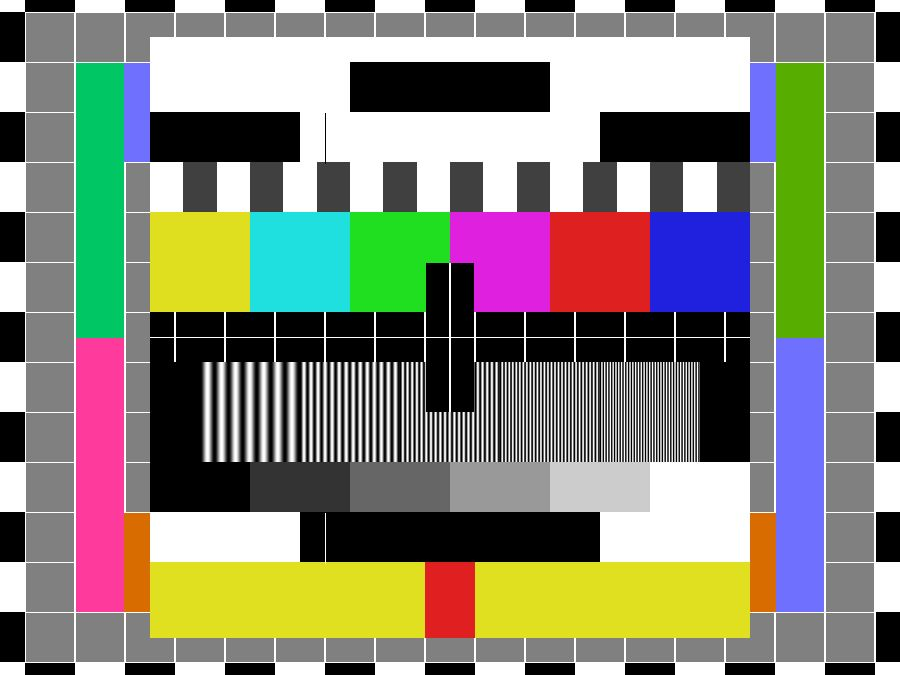
\includegraphics[width=0.5\textwidth]{images/test_image}
%     \caption{Example sprint burndown chart}
% \end{figure}

\subsection{Sprint Retrospective}
We will discuss what went well with each Sprint and what were areas that needed improvement. At the end of each cycle, we will discuss how to do things differently to make the next cycle run smoother.  

\subsection{Individual Status Reports}
Individual status reports will be given verbally at each scrum meeting. Those who can't attend will be required to submit a written update.

\subsection{Engineering Notebooks}
Team will sign on each others.

\subsection{Closeout Materials}
Our closeout materials include a minimum of the following:\newline
-Working Smart Mirror system\newline
-Video demo of the working system\newline
-Some form of documentation\newline

\subsubsection{Web Page}
We will have a web page hosted by Github to showcase our project.

\subsubsection{Source Code}
Source code and its versions are managed with git. 

\subsubsection{Source Code Documentation}
All source code shall be uploaded to GitHub / BitBucket in a repository in order to maintain version control and integrity. Clone requests shall be granted for all team members but restricted for all else until a designated "turnover" point.

\subsubsection{Hardware Schematics}
   	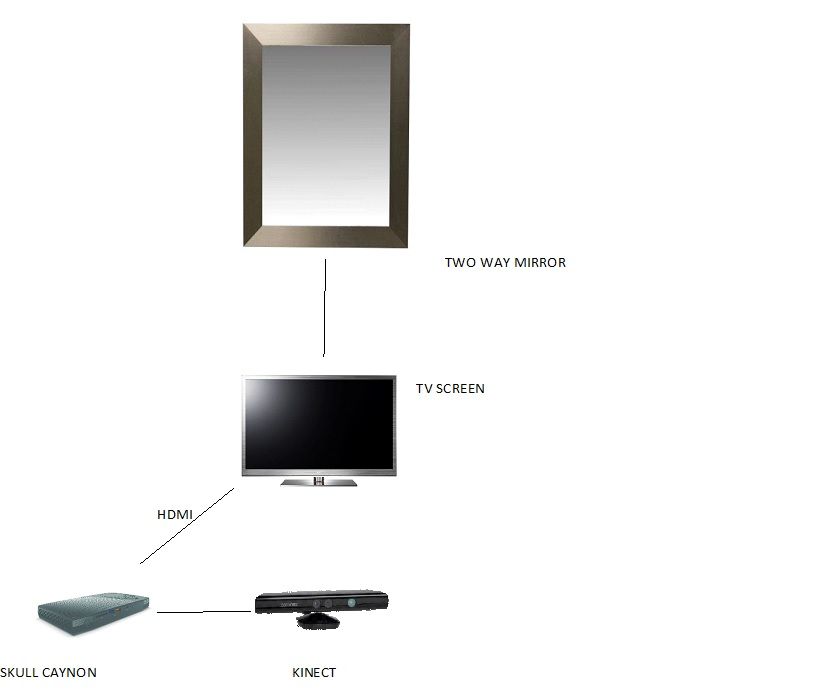
\includegraphics[width=0.90\textwidth]{images/Schematic}

\subsubsection{CAD files}
We will use Github to host our git repositories.

\subsubsection{Installation Scripts}
With the mirror as the hypothetical product, software would be preinstalled and ready for use out-of-the-box. As of our high-level definition, no installation scripts are defined. Live updates, modability, and manual installation will have to be of consideration later in the project, depending on the progress of crucial features.

\subsubsection{User Manual}
The user manual shall be comprised of Markdown text documents which shall be stored in the respective GitHub / BitBucket repository in order to maintain version control and integrity.